\chapter{Criptografía Simétrica. AES}
En este capítulo voy a explicar el cifrado Rijndael AES el cual es un cifrado de bloque simétrico muy utilizado actualmente por aplicaciones como \emph{Telegram}, \emph{WhatsApp} y \emph{FacebookChat} entre otras. Este algoritmo se usa principalmente para cifrar los mensajes ya que es muy eficiente a nivel computacional.\\
\section{El algoritmo Rijndael AES}
El algoritmo Rijndael llamado así en honor a sus dos autores Joan Daemen y Vicent Rijmen, es un algoritmo de cifrado por bloques que fue adoptado en octubre de 2000 por el NIST (\emph{National Institute for Standards and Technology}) para su empleo en aplicaciones criptográficas no militares en sustitución del algoritmo \emph{DES} después de un proceso de más tres años en los que se buscaba un algoritmo que fuera potente, eficiente y fácil de implementar.\\
Está diseñado para manejar longitudes de clave y de bloque variables entre los 128 y los 256 bits y aunque estos sean variables, en el estándar adoptado por el Gobierno de Estados Unidos en 2001 \cite{aesUsa} establece una longitud fija de bloque de 128 bits y una longitud de clave a escoger entre 128, 192 y 256 bits.\\
La información para los siguientes apartados de AES la he obtenido de \cite{En2011} y de \cite{criptografia}.
\newpage
\section{Estructura de AES}
AES es un algoritmo que se basa en aplicar un número determinado de rondas a un valor intermedio denominado \emph{estado} que puede ser representado por una matriz rectangular que posee cuatro filas y $N_{b}$ columnas. Análogamente, la clave tiene la misma estructura, una matriz de cuatro filas y $N_{k}$ columnas.
El bloque a cifrar o descifrar se traslada directamente byte a byte sobre la matriz de estado de columna en columna ($a_{0,0}, a_{1,0}, a_{2,0}, a_{3,0}, a_{0,1} \dots$).

\begin{table}[htb]
	\begin{center}
		\begin{tabular}{| c | c | c | c |}
				\hline
				$\math{a}_{0,0}$ & $\math{a}_{0,1}$ & $\math{a}_{0,2}$ & $\math{a}_{0,3}$\\ \hline
				$\math{a}_{1,0}$ & $\math{a}_{1,1}$ & $\math{a}_{1,2}$ & $\math{a}_{1,3}$\\ \hline
				$\math{a}_{2,0}$ & $\math{a}_{2,1}$ & $\math{a}_{2,2}$ & $\math{a}_{2,3}$\\ \hline
				$\math{a}_{3,0}$ & $\math{a}_{3,1}$ & $\math{a}_{3,2}$ & $\math{a}_{3,3}$\\ \hline
		\end{tabular}
		\caption{Ejemplo de matriz de estado con $N_b=4$(128 bits).}
	\end{center}
\end{table}

\begin{table}[htb]
	\begin{center}
		\begin{tabular}{| c | c | c | c |}
				\hline
				$\math{k}_{0,0}$ & $\math{k}_{0,1}$ & $\math{k}_{0,2}$ & $\math{k}_{0,3}$\\ \hline
				$\math{k}_{1,0}$ & $\math{k}_{1,1}$ & $\math{k}_{1,2}$ & $\math{k}_{1,3}$\\ \hline
				$\math{k}_{2,0}$ & $\math{k}_{2,1}$ & $\math{k}_{2,2}$ & $\math{k}_{2,3}$\\ \hline
				$\math{k}_{3,0}$ & $\math{k}_{3,1}$ & $\math{k}_{3,2}$ & $\math{k}_{3,3}$\\ \hline
		\end{tabular}
		\caption{Ejemplo de clave con $N_k=4$(128 bits).}
	\end{center}
\end{table}

En otros casos el bloque y la clave pueden ser representados como vectores de registro de 32 bits, donde cada registro esta compuesto por los bytes de la columna correspondiente ordenados en orden descendiente.\\

Siendo $B$ el bloque que queremos cifrar y $S$ la matriz de estado, el algoritmo AES con $n$ rondas se resume en:

\begin{enumerate}
	\item Calcular $K_0, K_1,...,K_n$ subclaves a partar de la clave $K$.
	\item $S\leftarrow B \oplus K_0$.
	\item Para $i=1$ hasta $n$ hacer:
	\begin{description}
			\item Aplicar la ronda \emph{i}-ésima del algoritmo con la subclave $K_i$.
	\end{description}
\end{enumerate}
Como las funciones usadas en cada ronda son invertibles, para descifrar aplicaremos las funciones inversas de las funciones usadas para cifrar en el orden opuesto.

\begin{table}[htb]
	\begin{center}
		\begin{tabular}{| c | c | c | c |}
				\hline
				& $N_b = 4$(128 bits) & $N_b = 6$(192 bits)& $N_b = 8$(256 bits)\\ \hline
				$N_k = 4$(128 bits)& 10 & 12 & 14\\ \hline
				$N_k = 6$(128 bits)& 12 & 12 & 14\\ \hline
				$N_k = 8$(128 bits)& 14 & 14 & 14\\ \hline
		\end{tabular}
		\caption{Número de rondas en función del tamaño de la clave y bloque.}
		\label{rondas_aes}
	\end{center}
\end{table}

En el algoritmo AES se define cada ronda como una composición de cuatro funciones invertibles diferentes, formando tres \emph{capas}. Estas funciones tienen un propósito específico.
\begin{itemize}
	\item \textbf{Capa de mezcla lineal:} formada por las funciones \emph{DesplazarFila} y \emph{MezclarColumnas} que permite obtener un alto nivel de difusión a lo largo de varias rondas.
	\item \textbf{Capa no lineal:} formada por la función \emph{ByteSub} y es la aplicación paralela de s-cajas con propiedades óptimas de no linealidad.
	\item \textbf{Capa de adición de clave:} es un simple \emph{o-exclusivo} entre el estado intermedio y la subclave correspondiente a cada ronda.
\end{itemize}

%\newpage
\section{Las Rondas de AES}
Una vez visto algunas de las propiedades de los cuerpos finitos, ya disponemos de las herramientas necesarias para describir las rondas de AES.
Dado que este algoritmo puede aplicarse para longitudes diferentes de bloque y clave, el número de rondas es variable, como se ha visto en \ref{rondas_aes}.\\
Siendo $S$ la matriz de estado y $K_i$ la subclave correspondiente a la ronda $i$-ésima, cada ronda posee esta estructura:
\begin{enumerate}
	\item $S \leftarrow ByteSub(S)$,
	\item $S \leftarrow DesplazarFila(S)$,
	\item $S \leftarrow MezclarColumnas(S)$,
	\item $S \leftarrow K_i \oplus S$.
\end{enumerate}
En la última ronda se hacen solo los tres primeros pasos del algoritmo.

	\subsubsection{ByteSub}
		La función \emph{ByteSub} es una sustitución no lineal que se aplica a cada byte de la matriz de estado mediante una s-caja 8\texttimes8. Se obtiene componiendo dos transformaciones:
		\begin{enumerate}
			\item Cada byte se considera como un elemento del $\operatorname{GF}(2^8)$ generado por el polinomio irreducible $m(x)=x^8+x^4+x^3+x+1$ y es sustituido por su inversa multiplicativa quedando el valor cero inalterado. 
			\item A continuación se aplica la siguiente transformación afín en $\operatorname{GF}(2^8)$ siendo $x_0, x_1,...,x_7$ los bits del byte correspondiente e $y_0, y_1,...,y_7$ los del resultado:

				\begin{equation*} 
					\begin{bmatrix} 
						y_0\\
						y_1\\
						y_2\\
						y_3\\
						y_4\\
						y_5\\
						y_6\\
						y_7\\
					\end{bmatrix}
					=
					\begin{bmatrix} % O matrices como esta de 4 x 3
						1 & 0 & 0 & 0 & 1 & 1 & 1 & 1\\
						1 & 1 & 0 & 0 & 0 & 1 & 1 & 1\\
						1 & 1 & 1 & 0 & 0 & 0 & 1 & 1\\
						1 & 1 & 1 & 1 & 0 & 0 & 0 & 1\\
						1 & 1 & 1 & 1 & 1 & 0 & 0 & 0\\
						0 & 1 & 1 & 1 & 1 & 1 & 0 & 0\\
						0 & 0 & 1 & 1 & 1 & 1 & 1 & 0\\
						0 & 0 & 0 & 1 & 1 & 1 & 1 & 1\\
					\end{bmatrix}
					\begin{bmatrix}
						x_0\\
						x_1\\
						x_2\\
						x_3\\
						x_4\\
						x_5\\
						x_6\\
						x_7\\
					\end{bmatrix}
					+
					\begin{bmatrix}
						1\\
						1\\
						0\\
						0\\
						0\\
						1\\
						1\\
						0\\
					\end{bmatrix}
			\end{equation*}
		\end{enumerate}
		La función inversa de $ByteSub$ es la aplicación inversa de la s-caja de cada byte de la matriz de estado.

	\subsubsection{DesplazarFila}
		Esta función desplaza a la izquierda de manera cíclica las filas de la matriz de estado. Cada fila $f_i$ se desplaza un número de posiciones $c_i$ diferente. Mientras que $c_0$ siempre es igual a cero, el resto de valores vine en función de $N_b$ como se puede ver en \ref{ciennb}.\\
		La función inversa será el desplazamiento de las filas de la matriz el mismo número de posiciones pero en el sentido contrario.

		\begin{table}[htb]
			\begin{center}
				\begin{tabular}{| c | c | c | c |}
						\hline
						$N_b$ & $c_1$ & $c_2$ & $c_3$\\ \hline
						4 & 1 & 2 & 3\\ \hline 
						6 & 1 & 2 & 3\\ \hline 
						8 & 1 & 3 & 4\\ \hline 
				\end{tabular}
				\caption{Valores de $c_i$ según el tamaño de bloque $N_b$}
				\label{ciennb}
			\end{center}
		\end{table}

		\begin{figure}[htb]
			\centering
			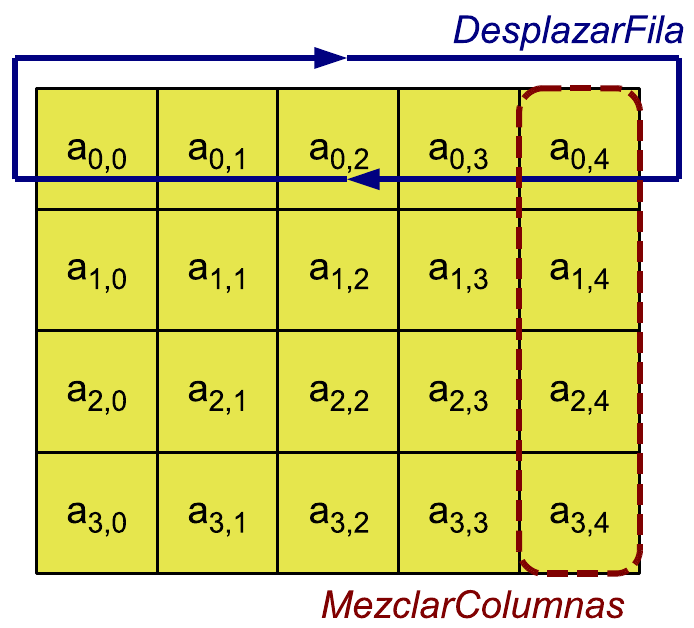
\includegraphics[scale=0.4]{imagenes/aesdesplazarmezclar.png} 
			\caption{Esquema de las funciones $MezclarColumnas$ y $DesplazarFila$ \cite{En2011}}
			\label{desplazarymezclar}
		\end{figure}
%\newpage
	\subsubsection{MezclarColumnas}
	Durante la aplicación de esta función cada columna del vector de estado es vista como una matriz $4 \times 1$ donde sus coeficientes pertenecen a $\mathbb{F}_{256}$. Aplicar MezclarColumnas a cada estado equivale a multiplicar cada columna por la matriz $4 \times 4$.

			\begin{center}
					\begin{pmatrix} 
						02 & 03 & 01 & 01 \\
						01 & 02 & 03 & 01 \\
						01 & 01 & 02 & 03 \\
						03 & 01 & 01 & 02 \\
					\end{pmatrix}
			\end{center}

\section{Cálculo de las Subclaves}
Las subclaves $K_i$ se obtienen de la clave principal $K$ mediante el uso de dos funciones: una de expansión y otra de selección. Siendo $n$ el número de rondas que se van a aplicar, la función de expansión obtiene a partir del valor de $K$ una secuencia de $4(n+1)N_b$ bytes.\\
La función de selección toma consecutivamente de la secuencia obtenida bloques del mismo tamaño que la matriz de estado y los asigna a cada $K_i$.\\

Sea $K(i)$ un vector de bytes de tamaño $4N_k$ conteniendo la clave y sea $W(i)$ un vector de $N_b(n+1)$ registros de 4 bytes, siendo $n$ el número de rondas. 
La función de expansión tiene dos versiones según el valor de $N_k$:

\begin{itemize}
	\item Si $N_k\le6$:
	\begin{algorithm}
		Para $i$ desde 0 hasta $N_{k}-1$ hacer:
		\begin{description}
			$W(i)\leftarrow(K(4·i), K(4·i+1), K(4·i+2), K(4·i+3))$
		\end{description}
		Para $i$ desde $N_k$ hasta $N_{b}·(n+1)$ hacer:\\
			\hspace*{20}$tmp\leftarrow W(i-1)$\\
			\hspace*{20}Si $i \mod N_k = 0$\\
			\hspace*{40}$tmp\leftarrow Sub(Rot(tmp))\oplus Rc(i/N_k)$\\
			\hspace*{20}$W(i)\leftarrow W(i-N_k)\oplus tmp$
	\end{algorithm}
%\newpage
	\item Si $N_k>6$:
	\begin{algorithm}
		Para $i$ desde 0 hasta $N_{k}-1$ hacer:
		\begin{description}
			$W(i)\leftarrow(K(4·i), K(4·i+1), K(4·i+2), K(4·i+3))$
		\end{description}
		Para $i$ desde $N_k$ hasta $N_{b}·(n+1)$ hacer:\\
			\hspace*{20}$tmp\leftarrow W(i-1)$\\
			\hspace*{20}Si $i \mod N_k = 0$\\
			\hspace*{40}$tmp\leftarrow Sub(Rot(tmp))\oplus Rc(i/N_k)$\\
			\hspace*{20}Si $i \mod N_k = 4$\\
			\hspace*{40}$tmp\leftarrow Sub(tmp)$\\
			\hspace*{20}$W(i)\leftarrow W(i-N_k)\oplus tmp$
	\end{algorithm}
\end{itemize}

La función \emph{Sub} devuelve el resultado de aplicar la s-caja de AES a cada uno de los bytes del registro de cuatro que se le pasa como parámetro, la función \emph{Rot} desplaza a la izquierda los bytes del registro y \emph{Rc(j)} es una constante que se define como:
\begin{itemize}
	\item $Rc(j)=(R(j),0,0,0)$.
	\item Cada $R(i)$ es el elemento de $\operatorname{GF}(2^8)$ correspondiente al valor $x^{i-1}$ módulo $x^8+x^4+x^3+x+1$.
\end{itemize}

